% -*- coding: utf-8 -*-

\begin{chapter}{Ветровая циркуляция}\label{chap:11}
% \chapter{Wind Driven Ocean Circulation} 
Что приводит в движение океанские течения? Ответом, который напрашивается
прежде всех остальных, будет: ветер. Однако, некоторые дополнительные 
размышления над этим вопросом могут привести к выводу, что все не так очевидно.
Мы могли бы отметить, например, что сильные течения, такие как 
экваториальные противотечения в Атлантическом и Тихом океанах, 
движутся против ветра. Испанские мореплаватели XVI~ст.\ обнаружили у
побережья Флориды сильные течения в северном направлении, которые не были
явно связаны с ветром. Как такое может происходить? Кроме того, почему сильные
течения были открыты у восточных побережий материков, но не у западных?
%
% What drives the ocean currents? At first, we might answer, the
% winds. But if we think more carefully about the question, we might not
% be so sure. We might notice, for example, that strong currents, such
% as the North Equatorial Countercurrents in the Atlantic and Pacific
% Ocean go upwind. Spanish navigators in the 16th century noticed strong
% northward currents along the Florida coast that seemed to be unrelated
% to the wind. How can this happen? And, why are strong currents found
% offshore of east coasts but not offshore of west coasts?

Ответы на эти вопросы были даны в трех выдающихся работах, опубликованных
в~1947--1951~гг. Харальд Свердруп показал в первой из них, что циркуляция
в верхнем километровом слое океана прямо зависит от ротора поля ветрового
напряжения\index{ветровое напряжение!ротор}, если сила Кориолиса изменяется
с широтой (Sverdrup, 1947). Генри Стоммел установил, что асимметрия
океанских круговоротов также определяется вариацией силы Кориолиса 
с широтой (Stommel, 1948). Наконец, Уолтер Манк учёл влияние 
eddy viscosity и вычислил циркуляцию в верхних слоях Тихого 
океана (Munk, 1950). Совместные достижения этих трех океанологов 
стали основой современной теории океанской циркуляции.
%
% Answers to the questions can be found in a series of three remarkable
% papers published from 1947 to 1951. In the first, Harald Sverdrup
% (1947) showed that the circulation in the upper kilometer or so of the
% ocean is directly related to the curl of the wind stress\index{wind
% stress!curl of} if the Coriolis force varies with latitude. Henry
% Stommel (1948) showed that the circulation in oceanic gyres is
% asymmetric also because the Coriolis force varies with
% latitude. Finally, Walter Munk (1950) added eddy viscosity and
% calculated the circulation of the upper layers of the
% Pacific. Together the three oceanographers laid the foundations for a
% modern theory of ocean circulation.

\begin{section}{Теория океанской циркуляции Свердрупа}\label{sec:SverdrupTheory}
% \section{Sverdrup's Theory of the Oceanic Circulation}
\index{Свердрупа теория}\index{океанская циркуляция!Свердрупа теория}%
\index{циркуляция!Свердрупа теория}В ходе анализа наблюдений за экваториальными
течениями, Свердруп пришел к соотношению~(\ref{eq:11.6}), которое связывает
ротор поля ветрового напряжения\index{ветровое напряжение!ротор} с переносом
массы\index{перенос!Свердрупа} в верхних слоях океана. Чтобы вывести это
соотношение, Свердруп предположил, что течение установившееся, 
боковое трение, молекулярная вязкость
и нелинейные члены уравнения движения, такие
как~$u\, \partial{u} / \partial{x}$, малы, 
а приповерхностная турбулентность\index{турбулентность!напряжение} 
может быть выражена через вертикальную турбулентную вязкость. 
Кроме того, было сделано предположение, что ветровая циркуляция 
прекращается при достижении некоторого уровня отсутствия движения.
С учетом этих предположений, горизонтальные составляющие уравнения
количества движения~\ref{??} и~\ref{??} принимают вид:
\begin{subequations}\label{eq:11.1}
\begin{equation}
 \frac{\partial{p}}{\partial{x}} 
    =  f\,\rho\,v + \frac{\partial{T_{xz}}}{\partial{z}},
\end{equation}
\begin{equation}
  \frac{\partial{p}}{\partial{y}} 
    = -f\,\rho\,u + \frac{\partial{T_{yz}}}{\partial{z}}.
\end{equation}
\end{subequations}
%
% \index{Sverdrup's Theory}\index{oceanic circulation!Sverdrup's
% Theory}\index{circulation!Sverdrup's Theory}While Sverdrup was
% analyzing observations of equatorial currents, he came upon (11.6)
% below relating the curl of the wind stress\index{wind stress!curl of}
% to mass transport\index{transport!Sverdrup} within the upper ocean. To
% derive the relationship, Sverdrup assumed that the flow is stationary,
% that lateral friction and molecular viscosity are small, that
% non-linear terms such as $u\, \partial{u} / \partial{x}$ are small,
% and that turbulence\index{turbulent!stress} near the sea surface can
% be described using a vertical eddy viscosity. He also assumed that the
% wind-driven circulation vanishes at some depth of no motion. With
% these assumptions, the horizontal components of the momentum equation
% from 8.9 and 8.12 become:
% \begin{subequations}
% \begin{equation}
% \frac{\partial{p}}{\partial{x}} =  f\,\rho\,v + \frac{\partial{T_{xz}}}{\partial{z}}
% \end{equation}
% \begin{equation}
% \frac{\partial{p}}{\partial{y}} = -f\,\rho\,u + \frac{\partial{T_{yz}}}{\partial{z}}
% \end{equation}
% \end{subequations}

Свердруп проинтегрировал эти уравнения от поверхности до глубины~$-D$, равной
или большей глубины, на которой горизонтальный градиент давления обращается
в нуль, и ввел следующие обозначения:
\begin{subequations}\label{eq:11.2}
\begin{alignat}{2}
\frac{\partial{P}}{\partial{x}} 
   &= \int\limits_{-D}^{0} \frac{\partial{p}}{\partial{x}}\,dz,  
&\qquad \frac{\partial{P}}{\partial{y}} 
   &= \int\limits_{-D}^{0} \frac{\partial{p}}{\partial{y}}\,dz,  \\
M_x 
   &\equiv \int\limits_{-D}^{0} \rho\,u(z)\,dz,          
&\qquad M_y 
   &\equiv \int\limits_{-D}^{0} \rho\,v(z)\,dz,
\end{alignat}
\end{subequations}
где~$M_x, M_y$~--- две компоненты переноса массы\index{перенос!Свердрупа}
в слое, подверженном влиянию ветра, нижней границей которого является
гипотетический уровень отсутствия движения.
%
% Sverdrup integrated these equations from the surface to a depth $-D$
% equal to or greater than the depth at which the horizontal pressure
% gradient becomes zero. He defined:
% \begin{subequations}
% \begin{alignat}{2}
% \frac{\partial{P}}{\partial{x}} &= \int\limits_{-D}^{0} \frac{\partial{p}}{\partial{x}}\,dz,  &\qquad
% \frac{\partial{P}}{\partial{y}} &= \int\limits_{-D}^{0} \frac{\partial{p}}{\partial{y}}\,dz,  \\
% M_x &\equiv \int\limits_{-D}^{0} \rho\,u(z)\,dz,          &\qquad M_y &\equiv \int\limits_{-D}^{0} \rho\,v(z)\,dz,
% \end{alignat}
% \end{subequations}
% where $M_x, M_y$ are the mass transports\index{transport!Sverdrup} in
% the wind-driven layer extending down to an assumed depth of no motion.

Горизонтальные граничные условия на морской поверхности задаются ветровым
напряжением\index{ветровое напряжение}. На глубине~$-D$ напряжение равно нулю
в силу того, что течение отсутствует:
\begin{alignat}{2}\label{eq:11.3}
 T_{xz}(0) &= T_x & \qquad T_{xz}(-D) &= 0, \notag \\
 T_{yz}(0) &= T_y & \qquad T_{yz}(-D) &= 0,
\end{alignat}
где~$T_x$ и~$T_y$~--- компоненты ветрового напряжения%
\index{ветровое напряжение!компоненты}.
%
% The horizontal boundary condition at the sea surface is the wind
% stress\index{wind stress}. At depth $-D$ the stress is zero because
% the currents go to zero:
% \begin{alignat}{2}
% T_{xz}(0) &= T_x & \qquad T_{xz}(-D) &= 0
% \notag \\
% T_{yz}(0) &= T_y & \qquad T_{yz}(-D) &= 0
% \end{alignat}
% where $T_x$ and $T_y$ are the components of the wind stress\index{wind
% stress!components}.

С учётом этих определений и граничных условий, уравнение~(\ref{eq:11.1}) 
принимает вид:
\begin{subequations}\label{eq:11.4}
\begin{align}
 \frac{\partial{P}}{\partial{x}} &= f\,M_y + T_x  \label{eq:11.4a}\\
 \frac{\partial{P}}{\partial{y}} &= -f\,M_x + T_y \label{eq:11.4b}
\end{align}
\end{subequations}
%
% Using these definitions and boundary conditions, (11.1) become:
% \begin{subequations}
% \begin{align}
% \frac{\partial{P}}{\partial{x}} &= f\,M_y + T_x  \\
% \frac{\partial{P}}{\partial{y}} &= -f\,M_x + T_y
% \end{align}
% \end{subequations}

Действуя аналогично, Свердруп проинтегрировал уравнение 
неразрывности~(\ref{eq:7.19}) по вертикали в тех же пределах, предполагая,
что вертикальная скорость на поверхности и на глубине~$-D$ равны нулю:
\begin{equation}\label{eq:11.5}
\frac{\partial{M_x}}{\partial{x}} + \frac{\partial{M_y}}{\partial{y}} = 0.
\end{equation}
%
% In a similar way, Sverdrup integrated the continuity equation (7.19)
% over the same vertical depth, assuming the vertical velocity at the
% surface and at depth $-D$ are zero, to obtain:
% \begin{equation}
% \frac{\partial{M_x}}{\partial{x}} + \frac{\partial{M_y}}{\partial{y}} = 0
% \end{equation}

Если продифференцировать~(\ref{eq:11.4a}) по переменной $y$ 
а~(\ref{eq:11.4b})~--- по~$x$, затем найти их разность и 
воспользоваться~(\ref{eq:11.5}), то мы получим:
\begin{align}\label{eq:11.6}
\beta\,M_y 
   &= \frac{\partial{T_y}}{\partial{x}} - \frac{\partial{T_x}}{\partial{y}},\notag \\
\beta\,M_y 
   &= \rot_z(T),
\end{align}
где $\beta \equiv \partial{f}/\partial{y}$~--- скорость изменения параметра
Кориолиса с широтой, а $\rot_z(T)$~--- вертикальная компонента ротора
ветрового напряжения\index{ветровое напряжение!ротор}.
%
% Differentiating (11.4a) with respect to $y$ and (11.4b) with respect
% to $x$, subtracting, and using (11.5) gives:
% \begin{align}
% \beta\,M_y &= \frac{\partial{T_y}}{\partial{x}} - \frac{\partial{T_x}}{\partial{y}}
% \notag \\
% \beta\,M_y &= \text{curl}_z(T)
% \end{align}
% where $\beta \equiv \partial{f}/\partial{y}$ is the rate of change of
% Coriolis parameter with latitude, and where curl$_z(T)$ is the
% vertical component of the curl of the wind stress\index{wind
% stress!curl of}.

Выше был получен очень важный фундаментальный результат: перенос массы 
ветровыми течениями в северном 
направлении\index{перенос!в северном направлении} равен ротору ветрового
напряжения. Отметим, что Свердруп допустил зависимость~$f$ от широты. Далее
будет показано, почему это принципиально.
%
% This is an important and fundamental result---the northward mass
% transport\index{transport!northward} of wind driven currents is equal
% to the curl of the wind stress. Note that Sverdrup allowed $f$ to vary
% with latitude. We will see later that this is essential.

Чтобы вычислить~$\beta $, можно воспользоваться соотношением
\begin{equation}\label{eq:11.7}
\beta \equiv \frac{\partial{f}}{\partial{y}} 
  = \frac{2\,\Omega\cos\varphi}{R},
\end{equation}
где $R$~--- радиус Земли, а~$\varphi$~--- широта.
%
% We calculate $\beta $ from
% \begin{equation}
% \beta \equiv \frac{\partial{f}}{\partial{y}} = \frac{2\,\Omega\cos\varphi}{R}
% \end{equation}
% where $R$ is earth's radius and $\varphi$ is latitude.

Направление ветров над большей частью поверхности открытого океана 
(особенно в тропиках) имеет зональный характер, так что
величина~$\partial{T_y}/\partial{x}$ достаточно мала, и
\begin{equation}\label{eq:11.8}
 M_y \approx -\frac{1}{\beta}\,\frac{\partial T_x}{\partial y}.
\end{equation}
После подстановки~(\ref{eq:11.8}) в~(\ref{eq:11.5}), а также в предположении,
что $\beta$~зависит от широты, Свердруп получил
\begin{equation}
\frac{\partial{M_x}}{\partial{x}}
  =-\frac{1}{2\,\Omega\cos\varphi}
    \left(\frac{\partial{T_x}}{\partial{y}}\Tan\varphi 
      + \frac{\partial^2{T_x}}{\partial{y}^2}R \right).
\end{equation}
%
% Over much of the open ocean, especially in the tropics, the wind is
% zonal and $\partial{T_y}/\partial{x}$ is sufficiently small that
% \begin{equation}
% M_y \approx -\frac{1}{\beta}\,\frac{\partial T_x}{\partial y}
% \end{equation}
% Substituting (11.8) into (11.5), assuming $\beta$ varies with
% latitude, Sverdrup obtained:
% \begin{equation}
% \frac{\partial{M_x}}{\partial{x}}=-
% \frac{1}{2\,\Omega\cos\varphi}\left(\frac{\partial{T_x}}{\partial{y}}\tan\varphi +
% \frac{\partial^2{T_x}}{\partial{y}^2}R \right)
% \end{equation}

\begin{figure}[t!]
\makebox[120mm] [c]{\includegraphics{pics/sverdrupmap}}
\caption{Линии тока переноса массы\index{перенос!в Тихом океане} в восточной
части Тихого океана, вычисленные согласно теории Свердрупа на основе 
среднегодового ветрового напряжения\index{ветровое напряжение!среднегодовое}. 
Reid (1948).}
\label{fig:sverdrupmap}
\end{figure}
%
% \begin{figure}[t!]
% %\vspace{-1ex}
% \makebox[120mm] [c]{\includegraphics{sverdrupmap}}
% \centering
% \footnotesize
% Figure 11.1 Streamlines of \rule{0mm}{3ex}mass
% transport\index{transport!in Pacific} in the eastern Pacific
% calculated\\from Sverdrup's theory using mean annual wind
% stress\index{wind stress!annual average}. After Reid (1948).
%
% \label{fig:sverdrupmap}
% \vspace{-3ex}
% \end{figure}

Далее он интегрировал данное уравнение по восточной границе в направлении
север-юг при~$x = 0$, при этом полагая, что поток через границу
отсутствует, то есть, что $M_x = 0$ при~$x = 0$. В этом случае
\begin{equation}\label{eq:11.10}
M_x =- \frac{\Delta{x}}{2\,\Omega\cos\varphi}
       \left[ \left<\frac{\partial{T_x}}{\partial{y}}    \right > \Tan\varphi 
             +\left<\frac{\partial^2{T_x}}{\partial{y}^2} \right> R \right],
\end{equation}
где $\Delta x$~--- расстояние от восточной границы океанского бассейна,
а угловыми скобками обозначены зональные средние ветрового напряжения%
\index{ветровое напряжение!зональное среднее} (рис.~\ref{fig:sverdrupmap}).
%% Строго говоря, "brackets" это квадратные скобки (в амер. англ.), 
%% но по сути сказанного, среднее должно быть обозначено угловыми.
%
% Sverdrup integrated this equation from a north-south eastern boundary
% at $ x = 0$, assuming no flow into the boundary. This requires $M_x = 0$ 
% at $x = 0$. Then
% \begin{equation}
% M_x =- \frac{\Delta{x}}{2\,\Omega\cos\varphi}\left[ \left<
% \frac{\partial{T_x}}{\partial{y}}\right > \tan\varphi +
% \left< \frac{\partial^2{T_x}}{\partial{y}^2} \right> R \right]
% \end{equation}
% where $\Delta x$ is the distance from the eastern boundary of the
% ocean basin, and brackets indicate zonal averages of the wind
% stress\index{wind stress!zonal average} (figure 11.1).

Чтобы проверить свою теорию, Свердруп сравнил величины 
переноса\index{перенос!Свердрупа}, вычисленные по известным ветрам в восточной
части тропической зоны Тихого океана, с полученными по гидрографическим
данным\index{гидрографические данные!НИС Carnegie}, собранным
НИС~\textit{Carnegie} и~\textit{Bushnell} в октябре и ноябре
1928, 1929 и~1939~гг.\ между \latlon{34}{N} и~\latlon{10}{S}, а также
между~\latlon{80}{W} и~\latlon{160}{W}. 
На основе этих данных\index{гидрографические данные!и перенос Свердрупа} 
при помощи интегрирования от глубины~$D = -1000\m$ была вычислена величина~$P$. 
Результаты сравнения, приведенные на рис.~\ref{fig:windpacific}, показывают,
что при помощи данной теории можно не только вычислить с хорошей точностью
величины переносов на основе данных о ветре, но также и предсказать 
существование ветровых течений, движущихся против ветра.
%
% To test his theory, Sverdrup compared
% transports\index{transport!Sverdrup} calculated from known winds in
% the eastern tropical Pacific with transports calculated from
% hydrographic data\index{hydrographic data!from Carnegie} collected by
% the \textit{Carnegie} and \textit{Bushnell} in October and November
% 1928, 1929, and 1939 between 34\degrees N and 10\degrees S and between
% 80\degrees W and 160\degrees W. The hydrographic
% data\index{hydrographic data!and Sverdrup transport} were used to
% compute $P$ by integrating from a depth of $D = -1000$ m. The
% comparison, figures 11.2, showed not only that the transports can be
% accurately calculated from the wind, but also that the theory predicts
% wind-driven currents going upwind.

\begin{figure}[t!]
\makebox[120mm] [c]{\includegraphics{pics/sverdrup}}
\caption{Перенос массы\index{перенос!в Тихом океане} в восточной части Тихого
океана, вычисленный согласно теории Свердрупа на основе данных наблюдений
за ветром при помощи уравнений~(\ref{eq:11.8}) и~(\ref{eq:11.10}) 
(сплошные линии), а также на основе давления, рассчитанного по 
судовым гидрографическим данным\index{гидрографические данные!и перенос Свердрупа}
при помощи уравнения~(\ref{eq:11.4}) (точки). Перенос выражен
в тоннах в секунду через сечение шириной~$1\m$ от морской поверхности до 
глубины~$1\km$. Отметим разницу в масштабе~$M_y$ и~$M_x$. Reid (1948)}
\label{fig:windpacific}
\end{figure}
%
% \begin{figure}[t!]
% \makebox[120mm] [c]{\includegraphics{sverdrup}}
% \footnotesize
% Figure 11.2 Mass \rule{0mm}{3ex}transport\index{transport!in Pacific}
% in the eastern Pacific calculated from Sverdrup's theory using
% observed winds with 11.8 and 11.10 (solid lines) and pressure
% calculated from hydrographic data\index{hydrographic data!and Sverdrup
% transport} from ships with 11.4 (dots). Transport is in tons per
% second through a section one meter wide extending from the sea surface
% to a depth of one kilometer. Note the difference in scale between
% $M_y$ and $M_x$. After Reid (1948).
% \label{fig:windpacific}
% \vspace{-4ex}
% \end{figure}

\begin{paragraph}{Теория Свердрупа: комментарии}
% \paragraph{Comments on Sverdrup's Solutions}
\begin{enumerate}
\item 
Свердруп предположил\index{Свердрупа предположения}, что 
   i) внутренние потоки в океане являются геострофическими;
  ii) существует единый уровень отсутствия движения;
 iii) теория экмановского переноса\index{экмановский перенос} корректна.
(В данном пособии теория Экмана и геострофическое равновесие были
рассмотрены в гл.~\ref{chap:9} и~\ref{chap:10}, соответственно.) 
Сведения об уровне отсутствия движения в тропической зоне Тихого океана 
в настоящий момент не отличаются полнотой.
%
% \vitem Sverdrup assumed\index{Sverdrup's assumptions} i) The internal
% flow in the ocean is geostrophic; ii) there is a uniform depth of no
% motion; and iii) Ekman's transport\index{Ekman transport} is
% correct. I examined Ekman's theory in Chapter 9, and the geostrophic
% balance in Chapter 10. We know little about the depth of no motion in
% the tropical Pacific.

\item 
Полученное решение применимо лишь на восточной границе океанского бассейна,
поскольку $M_x$ увеличивается с ростом~$x$. Такой эффект объясняется тем,
что модель не учитывает влияние трения, которое в конечном итоге 
уравновешивает потоки, возникающие под действием ветра. 
Тем не менее, теория Свердрупа использовалась для описания глобальной 
системы поверхностных течений. 
Решения были получены для каждого океана на всём протяжении до их 
западных пределов. При этом для соблюдения закона сохранения массы 
введены переносы с севера на юг в тонком горизонтальном пограничном слое
(рис.~\ref{fig:sverdrupxport}).
%
% \vitem The solutions are limited to the east side of the ocean because
% $M_x$ grows with $x$. The result comes from neglecting friction which
% would eventually balance the wind-driven flow. Nevertheless, Sverdrup
% solutions have been used for describing the global system of surface
% currents. The solutions are applied throughout each basin all the way
% to the western limit of the basin.  There, conservation of mass is
% forced by including north-south currents confined to a thin,
% horizontal boundary layer (figure 11.3).

\item 
Модель допускает единственное граничное условие: отсутствие потока через
восточную границу. Более полное описание потоков требует более полных же
уравнений.
%
% \vitem Only one boundary condition can be satisfied, no flow through
% the eastern boundary. More complete descriptions of the flow require
% more complete equations.

\item 
Теория не охватывает вертикальное распределение течений.
%
% \vitem The solutions do not give the vertical distribution of the
% current.

\item 
Достигнутые результаты были получены на основе наблюдений, проведенных
в двух исследовательских рейсах, и усредненных данных о ветре, предполагающих
равновесное состояние. Последующие вычисления Литмаа, Маккриэри и~Мура,
в которых использовались более поздние данные о ветре, привели к решениям
с выраженной сезонной изменчивостью, которые хорошо согласуются с наблюдениями
при условии, что глубина уровня отсутствия движения принята равной~$500\m$.
При выборе иной глубины согласование результатов оставляет желать лучшего
(Leetmaa, McCreary and Moore, 1981).
%
% \vitem Results were based on data from two cruises plus average wind
% data assuming a steady state. Later calculations by Leetmaa, McCreary,
% and Moore (1981) using more recent wind data produces solutions with
% seasonal variability that agrees well with observations provided the
% level of no motion is at 500 m. If another depth were chosen, the
% results are not as good.

\item 
Тщательный анализ свидетельств в пользу выполнения в океане соотношения
Свердрупа, проведенный Вюншем (Wunsch 1996: \S 2.2.3), привел его к выводу,
что в настоящий момент мы не располагаем сведениями, достаточными для проверки
этой теории:
\begin{quote}
Данная продолжительная дискуссия не ставила своей целью опровержение 
соотношения Свердрупа. Напротив, была сделана попытка подчеркнуть существующий
в океанологии разрыв между правдоподобной и привлекательной теорией с одной
стороны и возможностью продемонстрировать ее применимость для получения
количественных характеристик реальных полей океанских течений. (Wunsch, 1996)
\end{quote}
%
% \vitem Wunsch (1996: \S 2.2.3) after carefully examining the evidence
% for a Sverdrup balance in the ocean concluded we do not have
% sufficient information to test the theory. He writes
% \begin{quote} \small
% The purpose of this extended discussion has not been to disapprove the
% validity of Sverdrup balance. Rather, it was to emphasize the gap
% commonly existing in oceanography between a plausible and attractive
% theoretical idea and the ability to demonstrate its quantitative
% applicability to actual oceanic flow fields.---Wunsch (1996).
% \end{quote}

\begin{figure}[t!]
\makebox[120mm] [c]{\includegraphics{pics/sverdrupxport}}
\caption{Проинтегрированный по вертикали глобальный
перенос Свердрупа\index{перенос!глобальный, Свердрупа}, рассчитанный по данным
о ветровом напряжении\index{ветровое напряжение!и перенос Свердрупа} 
Хеллермана и Розенштейна (Hellerman and Rosenstein, 1983). 
Шаг изолиний~--- $10\Sv$. (Tomczak and Godfrey, 1994: 46)}
\label{fig:sverdrupxport}
\end{figure}
%
% \begin{figure}[t!]
% \makebox[120mm] [c]{\includegraphics{sverdrupxport}}
% \footnotesize
% Figure 11.3 Depth-integrated \rule{0mm}{3ex}Sverdrup transport
% \index{transport!global Sverdrup} applied globally using the wind
% stress\index{wind stress!and Sverdrup transport} from Hellerman and
% Rosenstein (1983). Contour interval is 10 Sverdrups. After Tomczak and
% Godfrey (1994: 46).
% \label{fig:sverdrupxport}
% \vspace{-4ex}
% \end{figure}

Вюнш, однако, отмечал, что:
\begin{quote}
Соотношения Свердрупа занимают в теории океанской циркуляции настолько
важное место, что их корректность в большинстве обсуждений принимается 
без каких-либо обоснований, после чего на основе этих соотношений делаются
дальнейшие выводы о динамике более высокого порядка\dots{} 
важность соотношения Свердрупа трудно переоценить. (Wunsch, 1996).
\end{quote}
Отметим, что разрыв между теорией и практикой сокращается. Измерения среднего
напряжения в экваториальной зоне Тихого океана (Yu and McPhaden, 1999) 
показали, что потоки в этом регионе подчиняются соотношению Свердрупа.
%
% Wunsch, however, notes
% \begin{quote} \small
% Sverdrup's relationship is so central to theories of the ocean
% circulation that almost all discussions assume it to be valid without
% any comment at all and proceed to calculate its consequences for
% higher-order dynamics\dots it is difficult to overestimate the
% importance of Sverdrup balance.---Wunsch (1996).
% \end{quote}
% But the gap is shrinking. Measurements of mean stress in the
% equatorial Pacific (Yu and McPhaden, 1999) show that the flow there is
% in Sverdrup balance.
\end{enumerate}
\end{paragraph}

\begin{paragraph}{Линии тока, траектории, функции тока.}
% \paragraph{Stream Lines, Path Lines, and the Stream Function}
Прежде, чем мы продолжим наше обсуждение ветровой циркуляции в океане,
нам потребуется ввести понятия линий и функций тока
(Kundu, 1990: 51 \& 66).
%
% Before discussing more about the ocean's wind-driven circulation, we
% need to introduce the concept of stream lines and the stream function
% (see Kundu, 1990: 51 \& 66).

Состояние потока в некоторый момент времени может быть определено векторным
полем скорости в каждой точке пространства. 
\emph{Линией тока}\index{линия тока|textbf} называется кривая, в каждой
точке которой касательная совпадает с вектором скорости в данной точке.
Если течение не установилось, вид этих линий зависит от времени.
%
% At each instant in time, we can represent a flow field by a vector
% velocity at each point in space. The instantaneous curves that are
% everywhere tangent to the direction of the vectors are called the
% \textit{stream lines}\index{stream lines|textbf} of the flow. If the
% flow is unsteady, the pattern of stream lines change with time.

Путь, который проходит движущаяся частица жидкости (а вместе с ней и
дрейфующий буй в случае измерения течений по Лагранжу), в гидромеханике
принято называть \emph{траекторией}\index{траектория (частицы)|textbf}.
Линии тока установившегося течения совпадают с траекториями вовлеченных 
в него частиц; в противном случае, они различны.
%
% The trajectory of a fluid particle, the path followed by a Lagrangian
% drifter, is called the \textit{path line}\index{path line|textbf} in
% fluid mechanics. The path line is the same as the stream line for
% steady flow, and they are different for an unsteady flow.

Описание двумерных потоков несжимаемой жидкости может быть упрощено
введением \emph{функции тока}\index{функция тока|textbf}~$\psi$ 
следующего вида:
\begin{equation}\label{eq:11.11}
 u \equiv \frac{\partial{\psi}}{\partial{y}}, \qquad
 v \equiv -\frac{\partial{\psi}}{\partial{x}}.
\end{equation}
%
% We can simplify the description of two-dimensional, incompressible
% flows by using the \textit{stream function}\index{stream
% function|textbf} $\psi$ defined by:
% \begin{equation}
% u \equiv \frac{\partial{\psi}}{\partial{y}}, \qquad v \equiv -
% \frac{\partial{\psi}}{\partial{x}},
% \end{equation}

Понятие функции тока нашло широкое применение благодаря тому, что 
векторное поле скорости можно рассчитать на основе этой скалярной функции. 
Как следствие, уравнения некоторых потоков принимают более простую форму.
%
% The stream function is often used because it is a scalar from which
% the vector velocity field can be calculated. This leads to simpler
% equations for some flows.

Функции тока также полезны для визуализации потока. В каждый момент времени
поток параллелен линиям уровня~$\psi$. Следовательно, если поток 
установился, линии уровня функции тока соответствуют траекториям частиц 
жидкости.
%
% Stream functions are also useful for visualizing the flow. At each
% instant, the flow is parallel to lines of constant $\psi$. Thus if the
% flow is steady, the lines of constant stream function are the paths
% followed by water parcels.

Объёмный расход между двумя линиями тока установившегося потока 
равен~$d\psi$, а объёмный расход потока между двумя линиями тока~$\psi_1$ 
и~$\psi _2$ составляет~$\psi _1 - \psi _2$. Чтобы в этом убедиться,
рассмотрим произвольную линию, соединяющую две линии тока
(рис.~\ref{fig:volxportsketch}). Объёмный расход между линиями тока равен
%
% The volume rate of flow between any two stream lines of a steady flow
% is $d\psi$, and the volume rate of flow between two stream lines $\psi
% _1$ and $\psi _2$ is equal to $\psi _1 - \psi _2$. To see this,
% consider an arbitrary line $dx = (dx, dy)$ between two stream lines
% (figure 11.4). The volume rate of flow between the stream lines is:
%
\begin{figure}[t!]
\makebox[120mm] [c]{\includegraphics{pics/volxportsketch}}
\caption{Volume transport\index{transport!volume} между линиями тока
двумерного установившегося потока. (Kundu, 1990: 68).}
\label{fig:volxportsketch}
\end{figure}
%
% \begin{figure}[t!]
% \makebox[120mm] [c]{\includegraphics{volxportsketch}}
% \centering
% \footnotesize
% Figure 11.4 Volume transport\index{transport!volume}
% \rule{0mm}{3ex}between stream lines in a\\
% two-dimensional, steady flow. After Kundu (1990: 68).
%
% \label{fig:volxportsketch}
% \vspace{-4ex}
% \end{figure}
%
\begin{equation}
v\,dx+(-u)\,dy=-\frac{\partial{\psi}}{\partial{x}}\,dx-\frac{\partial{\psi}}{\partial{y}}\,dy=-d\psi,
\end{equation}
а объёмный расход между двумя линиями тока численно равен разности 
соответствующих им значений~$\psi$.
%
% \begin{equation}
% v\,dx+(-u)\,dy=-\frac{\partial{\psi}}{\partial{x}}\,dx-\frac{\partial{\psi}}{\partial{y}}\,dy=-d\psi
% \end{equation}
% and the volume rate of flow between the two stream lines is
% numerically equal to the difference in their values of $\psi$.

Применим изложенные выше понятия к картам топографии океанской поверхности,
построенным по данным спутниковой альтиметрии. В разд.~\ref{sec:10.3} были
введены соотношения~(\ref{eq:10.10}):
\begin{align}\label{eq:11.13}
 u_s &= -\frac{g}{f}\,\frac{\partial{\zeta}}{\partial{y}}, \notag \\
 v_s &= \frac{g}{f}\,\frac{\partial{\zeta}}{\partial{x}}.
\end{align}
Сравнивая~(\ref{eq:11.13}) с~(\ref{eq:11.11}), приходим к очевидному выводу,
что
\begin{equation}
 \psi = -\frac{g}{f}\,\zeta,
\end{equation}
а форма морской поверхности определяется функцией тока, умноженной на 
масштабный коэффициент~$g/f$. Обратившись к рис.~\ref{fig:sshmean} видим, 
что линии постоянной высоты являются линиями тока, а поток направлен вдоль 
этих линий. Поверхностный геострофический перенос%
\index{геострофический перенос}\index{перенос!геострофический, массы}
пропорционален перепаду высот и не зависит от расстояния между линиями тока.
Аналогичные утверждения справедливы и для рис.~\ref{fig:wyrtkiplot}, 
за исключением того, что перенос\index{перенос!поверхностный, массы}
задан относительно поверхности~$1000\dBar$, которая примерно соответствует
глубине в~$1\km$.
%
% Now, lets apply the concepts to satellite-altimeter maps of the
% oceanic topography. In \S 10.3 I wrote (10.10)
% \vspace{-1.5ex}
% \begin{align}
% u_s &= -\frac{g}{f}\,\frac{\partial{\zeta}}{\partial{y}} \notag \\
% v_s &= \frac{g}{f}\,\frac{\partial{\zeta}}{\partial{x}}
% \end{align}
% Comparing (11.13) with (11.11) it is clear that
% \begin{equation}
% \psi = -\frac{g}{f}\,\zeta
% \end{equation}
% and the sea surface is a stream function scaled by $g/f$. Turning to
% figure 10.5, the lines of constant height are stream lines, and flow
% is along the lines. The surface geostrophic
% transport\index{geostrophic transport}\index{transport!geostrophic
% mass} is proportional to the difference in height, independent of
% distance between the stream lines.  The same statements apply to
% figure 10.9, except that the transport\index{transport!surface mass}
% is relative to transport at the 1000 decibars surface, which is
% roughly one kilometer deep.

В дополнение к функции тока переноса объема (которую обычно для простоты 
называют просто <<функцией тока>>), океанологи также иногда пользуются функцией
тока переноса массы\index{перенос!функция тока}~$\Psi$:
\begin{equation}\label{eq:11.15}
 M_x \equiv  \frac{\partial{\Psi}}{\partial{y}}, \qquad 
 M_y \equiv -\frac{\partial{\Psi}}{\partial{x}},
\end{equation}
приведенной на рис.~\ref{fig:windpacific} и~\ref{fig:sverdrupxport}.
%
% In addition to the stream function, oceanographers use the
% mass-transport stream\index{transport!stream function} function $\Psi$
% defined by:
% \begin{equation}
% M_x \equiv \frac{\partial{\Psi}}{\partial{y}}, \qquad M_y \equiv -
% \frac{\partial{\Psi}}{\partial{x}}
% \end{equation}
% This is the function shown in figures 11.2 and 11.3.
\end{paragraph}
\end{section}

\begin{section}[Западные пограничные течения]{Теория западных пограничных течений Стоммела}
% \section[Western Boundary Currents]{Stommel's Theory of Western Boundary Currents}
\index{западные пограничные течения!Стоммела теория}\index{Стоммела теория}%
В то самое время, когда Свердруп приблизился к пониманию циркуляции в восточной
части Тихого океана, Стоммел добился аналогичного применительно к западным
пограничным течениям. Для изучения циркуляции в северной части Атлантического
океана он воспользовался фактически теми же самыми 
уравнениями, что и Свердруп Stommel (1948): (\ref{eq:11.1}), (\ref{eq:11.2}) 
и~(\ref{eq:11.3}), расширив их понятием bottom stress, 
proportional to velocity to (\ref{eq:11.3}):
\begin{subequations}
\begin{alignat}{2}
\left(A_z \frac{\partial{u}}{\partial{z}}\right)_0 &= -T_x =-F\cos(\pi \,y/b)& \qquad \left(A_z \frac{\partial{u}}{\partial{z}}\right)_D &= -R\,u, \\
\left(A_z \frac{\partial{v}}{\partial{z}}\right)_0 &= -T_y =0 & \qquad \left(A_z \frac{\partial{v}}{\partial{z}}\right)_D &= -R\,v,
\end{alignat}
\end{subequations}
где~$F$ и~$R$~--- константы.
%
% \index{western boundary currents!Stommels Theory}\index{Stommel's
% Theory}At the same time Sverdrup was beginning to understand
% circulation in the eastern Pacific, Stommel was beginning to
% understand why western boundary currents occur in ocean basins. To
% study the circulation in the north Atlantic, Stommel (1948) used
% essentially the same equations used by Sverdrup (11.1, 11.2, and 11.3)
% but he added a bottom stress proportional to velocity to (11.3):
% \begin{subequations}
% \begin{alignat}{2}
% \left(A_z \frac{\partial{u}}{\partial{z}}\right)_0 &= -T_x =-F\cos(\pi \,y/b)& \qquad \left(A_z \frac{\partial{u}}{\partial{z}}\right)_D &= -R\,u \\
% \left(A_z \frac{\partial{v}}{\partial{z}}\right)_0 &= -T_y =0 & \qquad \left(A_z \frac{\partial{v}}{\partial{z}}\right)_D &= -R\,v
% \end{alignat}
% \end{subequations}
% where $F$ and $R$ are constants.

Стоммелом были получены уравнения для установившегося потока воды с постоянной 
плотностью в объеме, ограниченном по горизонтали 
прямоугольником~$0\leq y\leq b$, $0\leq x\leq \lambda$, и с постоянной 
глубиной~$D$. Прежде всего, был рассмотрен частный случай отсутствия суточного
вращения Земли. Полученное решение определяло симметричное расположение 
потоков без ярко выраженных западных пограничных течений
(рис.~\ref{fig:stommelcurrents}, слева). Аналогичная картина наблюдалась
и для модели, дополненной суточным вращением с постоянной скоростью. Далее
Стоммел предположил, что сила Кориолиса зависит от широты, получив в итоге
модель с западной интенсификацией (рис.~\ref{fig:stommelcurrents}, справа). 
Также он сделал предположение, что концентрация линий тока в западной 
части области позволяет объяснить существование 
Гольфстрима\index{Гольфстрим!Стоммела теория}
именно зависимостью силы Кориолиса от широты. В данный момент нам известно,
что изменение силы Кориолиса с широтой необходимо для существования западных
пограничных течений, а также что различные другие модели потоков, использующие
различные (другие?) подходы для учета трения, порождают западные пограничные
%% different = различные или иные?
течения иной структуры. В работе Педлоски (Pedlosky, 1987, гл.~5) приводятся
весьма полезные краткие и математически точные описания различных теорий
западных пограничных течений.
%
% Stommel calculated steady-state solutions for flow in a rectangular
% basin $0\leq y\leq b$, $0\leq x\leq \lambda$ of constant depth $D$
% filled with water of constant density. His first solution was for a
% non-rotating earth. This solution had a symmetric flow pattern with no
% western boundary current (figure 11.5, left). Next, Stommel assumed a
% constant rotation, which again led to a symmetric solution with no
% western boundary current. Finally, he assumed that the Coriolis force
% varies with latitude. This led to a solution with western
% intensification (figure 11.5, right). Stommel suggested that the
% crowding of stream lines in the west indicated that the variation of
% Coriolis force with latitude may explain why the Gulf
% Stream\index{Gulf Stream!Stommel's theory for} is found in the
% ocean. We now know that the variation of Coriolis force with latitude
% is required for the existence of the western boundary current, and
% that other models for the flow which use different formulations for
% friction, lead to western boundary currents with different
% structure. Pedlosky (1987, Chapter 5) gives a very useful, succinct,
% and mathematically clear description of the various theories for
% western boundary currents.

Как будет показано в следующей главе, результаты Стоммела могут быть также
истолкованы в терминах завихренности: ветер порождает направленный по часовой
стрелке вращательный момент (завихренность), который должен быть скомпенсирован
противоположно направленным моментом, возникающим на западной границе.
%
% In the next chapter, we will see that Stommel's results can also be
% explained in terms of vorticity---wind produces clockwise torque
% (vorticity), which must be balanced by a counterclockwise torque
% produced at the western boundary.

\begin{figure}[h!]
\makebox[120mm] [c]{\includegraphics{pics/stommelcurrents}}
\caption{Функция тока для потока в бассейне согласно вычислениям 
Стоммела (Stommel, 1948).  
\textbf{Слева:} поток при отсутствии вращения или при вращении с постоянной
скоростью. 
\textbf{Справа:} поток в случае линейного изменения вращения с широтой~$y$.}
\label{fig:stommelcurrents}
\end{figure}
%
% \begin{figure}[h!]
% %\vspace{-1ex}
% \makebox[120mm] [c]{\includegraphics{stommelcurrents}}
% \footnotesize
% Figure 11.5 Stream function \rule{0pt}{3ex}for flow in a basin as
% calculated by Stommel (1948).  \textbf{Left:} Flow for non-rotating
% basin or flow for a basin with constant rotation. \textbf{Right:} Flow
% when rotation varies linearly with y.
% \label{fig:stommelcurrents}
% \vspace{-3ex}
% \end{figure}
\end{section}

\begin{section}{Теория Манка}\label{sec:MunksSolution}
% \section{Munk's Solution}
\index{Манка теория}Свердруп и Стоммел указали в своих работах ряд процессов,
играющих ведущую роль в возникновении ветровой циркуляции масштабов океанского
бассейна. На основе их достижений, дополненных данными Россби по 
боковой вихревой вязкости (Rossby, 1936), У.~Манком была сформулирована теория
циркуляции в масштабе океана (Munk, 1950).
Манк применил идею Свердрупа о вертикальном интегрировании переноса
массы над уровнем отсутствия движения. Этот подход упрощает математическую 
формулировку задачи. Кроме того, он лучше соответствует реальности, поскольку
океанские течения концентрируются в верхнем километровом слое океана, они
не баротропны и не зависят от глубины. Чтобы учесть в модели влияние трения,
Манк воспользовался боковым вихревым трением с постоянным 
значением~$A_H = A_x = A_y$. Уравнения~(\ref{eq:11.1}) при этом принимают вид:
\begin{subequations}
\begin{align}
\frac{1}{\rho}\, \frac{\partial{p}}{\partial{x}}
   &=\quad f \,v+\frac{\partial}{\partial{z}}\left(A_z\frac{\partial{u}}{\partial{z}}\right) 
      + A_H\,\frac{\partial^2{u}}{\partial{x}^2} 
      + A_H\,\frac{\partial^2{u}}{\partial{y}^2} \label{eq:11.17a}\\
\frac{1}{\rho}\, \frac{\partial{p}}{\partial{y}} 
   &=\:-f \,u+\frac{\partial}{\partial{z}}\left(A_z\frac{\partial{v}}{\partial{z}}\right) 
      + A_H\,\frac{\partial^2{v}}{\partial{x}^2} 
      + A_H\,\frac{\partial^2{v}}{\partial{y}^2} \label{eq:11.17b}
\end{align}
\end{subequations}
%
% \index{Munk's solution}Sverdrup's and Stommel's work suggested the
% dominant processes producing a basin-wide, wind-driven
% circulation. Munk (1950) built upon this foundation, adding
% information from Rossby (1936) on lateral eddy viscosity, to obtain a
% solution for the circulation within an ocean basin. Munk used
% Sverdrup's idea of a vertically integrated mass transport flowing over
% a motionless deeper layer. This simplified the mathematical problem,
% and it is more realistic. The ocean currents are concentrated in the
% upper kilometer of the ocean, they are not barotropic and independent
% of depth. To include friction, Munk used lateral eddy friction with
% constant $A_H = A_x = A_y$. Equations (11.1) become:
%
% \begin{subequations}
% \begin{align}
% \frac{1}{\rho}\, \frac{\partial{p}}{\partial{x}}
% &=\quad f \,v+\frac{\partial}{\partial{z}}\left(A_z
% \frac{\partial{u}}{\partial{z}}\right) + A_H\,
% \frac{\partial^2{u}}{\partial{x}^2} + A_H\, \frac{\partial^2{u}}{\partial{y}^2} \\
% \frac{1}{\rho}\, \frac{\partial{p}}{\partial{y}} &=\:-f \,u+\frac{\partial}{\partial{z}}\left(A_z
% \frac{\partial{v}}{\partial{z}}\right) + A_H\, \frac{\partial^2{v}}{\partial{x}^2} + A_H\,
% \frac{\partial^2{v}}{\partial{y}^2}
% \end{align}
% \end{subequations}

Манк интегрировал уравнения по вертикали от глубины~$-D$ до 
поверхности~$z = z_0$. Это напоминает подход Свердрупа, но с той разницей,
что в данном случае поверхность не совпадает с поверхностью океана~$z = 0$. 
Кроме того, были сделаны предположения, что течение на глубине~$-D$ отсутствует, 
условия~(\ref{eq:11.3}) применимы к горизонтальным границам на верхней и нижней
границах слоя, а величина~$A_H$ постоянна.
%
% Munk integrated the equations from a depth $-D$ to the surface at 
% $z = z_0$ which is similar to Sverdrup's integration except that the
% surface is not at $z = 0$.  Munk assumed that currents at the depth
% $-D$ vanish, that (11.3) apply at the horizontal boundaries at the top
% and bottom of the layer, and that $A_H$ is constant.

Чтобы упростить уравнения, Манк воспользовался функцией тока для переноса
массы\index{перенос!функция тока}~(\ref{eq:11.15}) и продолжил рассуждения
так, как это было ранее проделано Свердрупом. Продифференцировав 
уравнение~(\ref{eq:11.17a}) по переменной~$y$, 
а уравнение~(\ref{eq:11.17b})~--- по~$x$, можно тем самым избавиться от
слагаемого, представляющего давление, после чего уравнение переноса массы
принимает вид:
\begin{equation}\label{eq:11.18}
\underbrace{A_H \nabla^{4}\Psi\vphantom{\frac{\partial\Psi}{\partial{x}}}}_{\text{трение}}
 -\underbrace{\beta\,\frac{\partial\Psi}{\partial{x}} =-\rot_z T\,}_{\text{соотн. Свердрупа}},
\end{equation}
где
\begin{equation}
\nabla^4 =\frac{\partial^4}{\partial{x}^4}
          + 2\,\frac{\partial^4}{\partial{x}^2\,\partial{y}^2} 
          + \frac{\partial^4}{\partial{y}^4}
\end{equation}
называется бигармоническим оператором. Уравнение~(\ref{eq:11.18}) представляет
собой уравнение~(\ref{eq:11.6}), дополненное слагаемым, представляющим
боковое трение~$A_H$. Это слагаемое велико вблизи побережья, где 
горизонтальные производные поля скорости также велики, а во внутренних областях
океанского бассейна~--- мало. Таким образом, вдали от побережья соотношение
сил, вычисленное по данной методике, совпадает с результатами применения
уравнений Свердрупа.
%
% To simplify the equations, Munk used the mass-transport stream
% function\index{transport!stream function} (11.15), and he proceeded
% along the lines of Sverdrup. He eliminated the pressure term by taking
% the $y$ derivative of (11.17a) and the $x$ derivative of (11.17b) to
% obtain the equation for mass transport:
% \begin{equation}
% \underbrace{A_H \nabla^{4}
% \Psi\vphantom{\frac{\partial\Psi}{\partial{x}}}}_{\text{Friction}}\:-\:\underbrace{\beta\,\frac{\partial\Psi}{\partial{x}} =-\,\text{curl}_z T
% \,}_{\text{Sverdrup Balance}}
% \end{equation}
% where
% \begin{equation}
% \nabla^4 =\frac{\partial^4}{\partial{x}^4}+2\,\frac{\partial^4}{\partial{x}^2
% \,\partial{y}^2} + \frac{\partial^4}{\partial{y}^4}
% \end{equation}
% is the biharmonic operator. Equation (11.18) is the same as (11.6)
% with the addition of the lateral friction term $A_H$. The friction
% term is large close to a lateral boundary where the horizontal
% derivatives of the velocity field are large, and it is small in the
% interior of the ocean basin. Thus in the interior, the balance of
% forces is the same as that in Sverdrup's solution.

\begin{figure}[t!]
\includegraphics{pics/munkcurrents}
\caption{\textbf{Слева:} среднегодовое ветровое напряжение%
\index{ветровое напряжение!среднегодовое}~$T_x (y)$ над Тихим океаном 
и его ротор; $\varphi _b$~--- северная и южная границы круговоротов, 
где $M_y = 0$ и~$\rot\tau = 0$; $\varphi_0$~--- центр круговорота.  
\textbf{Справа вверху:} функция тока переноса массы\index{перенос!функция тока} 
для прямоугольной области, вычисленная Манком в работе (Munk 1950)  на основе
наблюдений за ветровым напряжением в Тихом океане. Изолинии проведены 
с шагом~$10\Sv$. Суммарный перенос от побережья до некоторой точки~$x,y$ 
составляет~$\psi (x,y)$. Величина переноса в сравнительно узком
северном секторе существенно преувеличена.
%% речь идет о неверных расчетах Манка или об утрированном масштабе?
\textbf{Справа внизу:} меридиональная составляющая переноса массы.
(Munk 1950)}
\label{fig:munkcurrents}
\end{figure}
%
% \begin{figure}[t!]
% \includegraphics{munkcurrents}
% \footnotesize
% Figure 11.6 \textbf{Left:} Mean \rule{0mm}{4ex}annual wind
% stress\index{wind stress!annual average} $T_x (y)$ over the Pacific
% and the curl of the wind stress. $\varphi _b$ are the northern and
% southern boundaries of the gyres, where $M_y = 0$ and curl $\tau = 0$.
% $\varphi _0$ is the center of the gyre.  \textbf{Upper Right:} The
% mass transport stream function\index{transport!stream function} for a
% rectangular basin calculated by Munk (1950) using observed wind stress
% for the Pacific. Contour interval is 10 Sverdrups. The total transport
% between the coast and any point $x,y$ is $\psi (x,y)$.The transport in
% the relatively narrow northern section is greatly exaggerated.
% \textbf{Lower Right:} North-South component of the mass
% transport. After Munk (1950).
% \label{fig:munkcurrents}
% \vspace{-3ex}
% \end{figure}

Уравнение~(\ref{eq:11.18}) представляет собой уравнение в частных производных
четвертого порядка, которому требуются четыре граничных условия. 
Манк предположил, что поток на границе параллелен этой границе, причем 
скольжение на границе отсутствует:
\begin{equation}\label{eq:11.20}
 \Psi_{\text{\textit{bdry}}} = 0, \qquad 
 \left(\frac{\partial{\Psi}}{\partial{n}}\right)_{\text{\textit{bdry}}} = 0,
\end{equation}
где $n$~--- нормаль к границе. Далее он воспользовался~(\ref{eq:11.20}),
чтобы решить~(\ref{eq:11.18}) в предположении, что поток заключен в 
прямоугольную область, границы которой составляют от~$x = 0$ до~$x = r$
и от~$y = -s$ до~$y = +s$, а также что ветровое 
напряжение\index{ветровое напряжение} имеет зональный характер и подчиняется
закону:
\begin{align}
 T&=a\,\cos ny + b\,\sin ny \,+\, c  \notag \\
 n&=j\,\pi/s, \qquad j=1,\,2,\,\dots
\end{align}
%
% Equation (11.18) is a fourth-order partial differential equation, and
% four boundary conditions are needed. Munk assumed the flow at a
% boundary is parallel to a boundary and that there is no slip at the
% boundary:
% \begin{equation}
% \Psi_{bdry} = 0, \qquad \left(\frac{\partial{\Psi}}{\partial{n}}\right)_{bdry} = 0
% \end{equation}
% where $n$ is normal to the boundary. Munk then solved (11.18) with
% (11.20) assuming the flow was in a rectangular basin extending from 
% $x = 0$ to $x = r$, and from $y = -s$ to $y = +s$. He further assumed
% that the wind stress\index{wind stress} was zonal and in the form:
% \begin{align}
% T&=a\,\cos ny + b\,\sin ny \,+\, c  \notag \\
% n&=j\,\pi/s, \qquad j=1,\,2,\,\dots
% \end{align}

Полученные результаты (рис.~\ref{fig:munkcurrents}) отображают основные
черты циркуляции масштаба океанских круговоротов. На востоке океанских
бассейнов она соответствует вычисленной Свердрупом, а в западной их части 
согласно теории должно существовать сильное пограничное течение. 
Положив~$A_H = 5 \times 10^{3}\sqmps$, получим приблизительную ширину
пограничного течения, которая составляет~$225\km$, а форма течения схожа
с потоками, наблюдаемыми в Гольфстриме и Куросио\index{Куросио!ширина}.
%
% Munk's solution (figure 11.6) shows the dominant features of the
% gyre-scale circulation in an ocean basin. It has a circulation similar
% to Sverdrup's in the eastern parts of the ocean basin and a strong
% western boundary current in the west. Using $A_H = 5 \times 10^{3}$
% m$^2$/s gives a boundary current roughly 225 km wide with a shape
% similar to the flow observed in the Gulf Stream and the
% Kuroshio\index{Kuroshio!width of}.

Величина переноса западных пограничных 
течений\index{перенос!западных пограничных течений} не зависит от~$A_H$, 
а определяется исключительно уравнением~(\ref{eq:11.6}), интегрированным
поперек океанского бассейна. Следовательно, она зависит от ширины океана,
ротора ветрового напряжения\index{ветровое напряжение!ротор} и~$\beta$. 
Используя лучшие оценки ветрового напряжения, доступные в то время,
Манк вычислил оценку величин переноса Гольфстрима%
\index{Гольфстрим!перенос}\index{перенос!Гольфстрима} 
и Куросио\index{Куросио!перенос}, которые 
составили~$36\Sv$ и~$39\Sv$ соответственно. Эти значения примерно в два раза
меньше результатов измерений, известных Манку. Такое соответствие следует
считать очень хорошим, если принять во внимание, что ветровое 
напряжение\index{ветровое напряжение} не было как следует изучено.
%
% The transport in western boundary currents\index{transport!in western
% boundary currents} is independent of $A_H$, and it depends only on
% (11.6) integrated across the width of the ocean basin. Hence, it
% depends on the width of the ocean, the curl of the wind
% stress\index{wind stress!curl of}, and $\beta$. Using the best
% available estimates of the wind stress, Munk calculated that the Gulf
% Stream\index{Gulf Stream!transport}\index{transport!by Gulf Stream}
% should have a transport of 36 Sv and that the
% Kuroshio\index{Kuroshio!transport of} should have a transport of 39
% Sv. The values are about one half of the measured values of the flow
% available to Munk. This is very good agreement considering the wind
% stress\index{wind stress} was not well known.

Более поздние попытки провести аналогичные вычисления также показали хорошее
соответствие теории наблюдениям за исключением области сильной рециркуляции
вблизи м.~Гаттерас. Результаты Манка были основаны на данных о ветровом
напряжении\index{ветровое напряжение}, осредненным по квадратам 
со стороной~$\degrees{5}$, следствием чего было занижение оценки ротора
ветрового напряжения. Литмаа и Bunker воспользовались современными данными
о коэффициенте трения\index{drag!коэффициент} и ветровым напряжением, 
осредненным по областям размером~$\degrees{2} \times \degrees{5}$, на основании
чего получили величину переноса Гольфстрима\index{Гольфстрим!перенос},
равную~$32\Sv$, что довольно близко к результату, вычисленному 
Манком (Leetmaa and Bunker, 1978).
%
% Recent recalculations show good agreement except for the region
% offshore of Cape Hatteras where there is a strong
% recirculation. Munk's solution was based on wind stress\index{wind
% stress} averaged aver 5\degrees squares. This underestimated the curl
% of the stress. Leetmaa and Bunker (1978) used modern drag
% coefficient\index{drag!coefficient} and 2\degrees $\times$ 5\degrees\
% averages of stress to obtain 32 Sv transport in the Gulf
% Stream\index{Gulf Stream!transport}, a value very close to that
% calculated by Munk.
\end{section}

\begin{section}{Поверхностная циркуляция в Атлантическом океане по данным наблюдений}
% \section{Observed Surface Circulation in the Atlantic}
Теории Свердрупа, Манка и Стоммела описывают идеализированные потоки. Однако,
реальный океан оказывается намного сложнее. Чтобы продемонстрировать, насколько
сложным может оказаться поверхностное течение, рассмотрим целый океанский
бассейн~--- северную часть Атлантического океана. Выбор этого региона 
обусловлен тем, что он лучше других покрыт наблюдениями, а также тем,
что процессы, происходящие в умеренных широтах Атлантического океана схожи
с аналогичными процессами в других океанах. Таким образом, в частности, 
Гольфстрим может использоваться в качестве примера западного пограничного
течения.
%
% The theories by Sverdrup, Munk, and Stommel describe an idealized
% flow. But the ocean is much more complicated. To see just how
% complicated the flow is at the surface, let's look at a whole ocean
% basin, the north Atlantic. I have chosen this region because it is the
% best observed, and because mid-latitude processes in the Atlantic are
% similar to mid-latitude processes in the other ocean. Thus, for
% example, I use the Gulf Stream as an example of a western boundary
% current.

На примере Гольфстрима\index{Гольфстрим!наблюдения} будет показано, 
как эволюционировали наши представления о поверхностных океанских течениях.
Безусловно, мы не в состоянии коснуться всех аспектов данной темы, поэтому
вынуждены предложить заинтересованному читателю обратиться к работам по
региональной океанографии, таким как (Tomczak and Godfrey, 1994).
%
% Let's begin with the Gulf Stream\index{Gulf Stream!observations of} to
% see how our understanding of ocean surface currents has evolved. Of
% course, we can't look at all aspects of theflow. You can find out much
% more by reading Tomczak and Godfrey (1994) book on\textit{Regional
% Oceanography: An Introduction}.

\begin{paragraph}{Североатлантическая циркуляция.}
% \paragraph{North Atlantic Circulation}
\index{циркуляция!североатлантическая}Среди всех океанских бассейнов наиболее
хорошо изученной считается северная часть Атлантического океана. Для этого
региона были разработаны развитые теории, охватывающие как поверхностные
течения, так и течения в слое термоклина\index{термоклин!север Атлантического океана}
и глубинную циркуляцию. Подкреплением этих теорий служит большой объем
данных, собранных в ходе многолетних наблюдений. Изучение иллюстраций, 
наглядно демонстрирующих характер циркуляции, может существенно помочь в её
понимании, при этом с точки зрения полноты картины предпочтительнее 
иллюстрации, построенные по данным за несколько последних десятилетий.
%
% \index{circulation!North Atlantic}The north Atlantic is the most
% thoroughly studied ocean basin. There is an extensive body of theory
% to describe most aspects of the circulation, including flow at the
% surface, in the thermocline\index{thermocline!in North Atlantic}, and
% at depth, together with an extensive body of field observations. By
% looking at figures showing the circulation, we can learn more about
% the circulation, and by looking at the figures produced over the past
% few decades we can trace an ever more complete understanding of the
% circulation.

Начнём наш обзор с традиционного изображения осредненных по времени 
поверхностных течений в северной части Атлантического океана, в основу которого
положены, главным образом, данные гидрографических наблюдений%
\index{гидрографические данные!и североатлантическая циркуляция}
полей плотности (рис.~\ref{fig:Fig2-8}). Это изображение соответствует
%% в оригинале рис. 2.7, но по смыслу именно 2.8.
современным представлениям об осредненной циркуляции в океане, 
основанным на данных, накопленных в течение более чем столетия наблюдений.
Может сложиться впечатление, что данная схема чрезмерно упрощена, поскольку
отображает весь мировой океан в целом. Во избежание подобных проблем,
ограничимся изображением осредненной циркуляции в северной части 
Атлантического океана (рис.~\ref{fig:NAtlcur1}).
%
% Let's begin with the traditional view of the time-averaged surface
% flow in the north Atlantic based mostly on hydrographic
% observations\index{hydrographic data!and north Atlantic circulation}
% of the density field (figure 2.7). It is a contemporary view of the
% mean circulation of the entire ocean based on a century of more of
% observations. Because the figure includes all the ocean, perhaps it is
% overly simplified. So, let's look then at a similar view of the mean
% circulation of just the north Atlantic (figure 11.7).

На этом рисунке изображен обширный круговорот, расположенный в умеренных 
широтах, ширина которого примерно равна ширине океанского бассейна,
а существование предсказано теорией Свердрупа 
(разд.~\ref{sec:SverdrupTheory}). В западной части находится западное
пограничное течение Гольфстрим%
\index{Гольфстрим!как западное пограничное течение}, которое замыкает
круговорот. Севернее расположен субполярный круговорот, включающий в себя
Лабрадорское течение. Система экваториальных течений и противотечений,
изображенная в нижней части рисунка в области низких широт, напоминает
аналогичные потоки, существующие в Тихом океане. Отметим, однако, наличие
на западе Атлантики сильного течения, движущегося вдоль северо-восточного 
побережья Бразилии к Карибскому морю и пересекающего экватор.
%
% The figure shows a broad, basin-wide, mid latitude gyre as we expect
% from Sverdrup's theory described in \S 11.1. In the west, a western
% boundary current, the Gulf Stream\index{Gulf Stream!as a western
% boundary current}, completes the gyre. In the north a subpolar gyre
% includes the Labrador current. An equatorial current system and
% countercurrent are found at low latitudes with flow similar to that in
% the Pacific. Note, however, the strong cross equatorial flow in the
% west which flows along the northeast coast of Brazil toward the
% Caribbean.

\begin{figure}[t!]
\makebox[121 mm] [c] {\includegraphics{pics/NAtlcur1}}
\caption{Схематическое изображение основных поверхностных течений в северной
части Атлантического океана. Числами обозначена величина 
переноса\index{перенос!север Атлантического океана}, выраженная 
в~$10^6\text{~м}^3/\text{с}$. (Sverdrup, Johnson, and Fleming, 1942: fig. 187).}
\label{fig:NAtlcur1}
\end{figure}
%
% \begin{figure}[t!]
% \makebox[121 mm] [c] {\includegraphics{NAtlcur1}}
% \centering
% \footnotesize
% Figure 11.7 Sketch \rule{0mm}{3ex}of the major surface currents in the
% North Atlantic. Values are transport\index{transport!in North
% Atlantic} in units of $10^6$ m$^3$/s. After Sverdrup, Johnson, and
% Fleming (1942: fig. 187).
%
% \label{fig:NAtlcur1}
% \vspace{-4ex}
% \end{figure}

\begin{figure}[t!]
\makebox[121 mm][c] {\includegraphics{pics/NATLcur}}
\caption{Подробная схема именованных течений в северной части 
Атлантического океана.
Числами обозначена величина переноса\index{перенос!северная Атлантика} 
в приповерхностном слое толщиной~$1\km$, выраженная в~$10^6\cubmps$.
\textbf{Eg}: Восточно-Гренландское течение; 
\textbf{Ei}: Восточно-Исландское течение; 
\textbf{Gu}: Гольфстрим\index{Гольфстрим};
\textbf{Ir}: течение Ирмингера; 
\textbf{La}: Лабрадорское течение;
\textbf{Na}: Северо-Атлантическое течение; 
\textbf{Nc}: Нордкапское течение;
\textbf{Ng}: Норвежское течение; 
\textbf{Ni}: Северо-Исландское течение;
\textbf{Po}: Португальское течение; 
\textbf{Sb}: Шпицбергенское течение;
\textbf{Wg}: Западно-Гренландское течение. 
Числами, заключенными в квадраты, обозначено опускание воды, выраженное 
в~$10^6\cubmps$. 
Теплые течения обозначены сплошными линиями, а холодные --- прерывистыми. 
(Dietrich et al., 1980:542).}
\label{fig:NATLcur1}
\end{figure}
%
% \begin{figure}[t!]
% \makebox[121 mm][c] {\includegraphics{NATLcur}}
% \footnotesize
% Figure 11.8 Detailed schematic \rule{0mm}{3ex}of named currents in the
% north Atlantic.  The numbers give the transport\index{transport!in
% North Atlantic} in units on $10^6 m^3/s$ from the surface to a depth
% of 1 km. \textbf{Eg}: East Greenland Current; \textbf{Ei}: East
% Iceland Current; \textbf{Gu}: Gulf Stream\index{Gulf Stream};
% \textbf{Ir}: Irminger Current; \textbf{La}: Labrador Current;
% \textbf{Na}: North Atlantic Current; \textbf{Nc}: North Cape Current;
% \textbf{Ng}: Norwegian Current; \textbf{Ni}: North Iceland Current;
% \textbf{Po}: Portugal Current; \textbf{Sb}: Spitsbergen Current;
% \textbf{Wg}: West Greenland Current. Numbers within squares give
% sinking water in units on $10^6 m^3 /s$. Solid Lines: Warmer
% currents. Broken Lines: Colder currents. After Dietrich et al. (1980:
% 542).
% \label{fig:NATLcur1}
% \vspace{-3ex}
% \end{figure}

Если мы ограничимся еще более узкой областью в северной части Атлантического 
океана (рис.~\ref{fig:NATLcur1}), то мы обнаружим, что картина течений
становится сложнее. Она включает в себя дополнительные подробности
по данному региону, представляющему особую важность для рыболовства и
торгового мореплавания. Можно ли утверждать, что эта схема, построенная
по самой полной базе гидрографических наблюдений, адекватно отображает 
реальность? В частности, если мы выпустим в океан измеритель течения
лагранжева типа, будет ли он следовать линиям тока, изображенным на рисунке?
%
% If we look closer at the flow in the far north Atlantic (figure 11.8)
% we see that the flow is still more complex. This figure includes much
% more detail of a region important for fisheries and commerce. Because
% it is based on an extensive base of hydrographic observations, is this
% reality? For example, if we were to drop a Lagrangian float into the
% Atlantic would it follow the streamline shown in the figure?

Чтобы ответить на этот вопрос, обратимся к работе Ф. Ричардсона, который
собрал данные о траекториях 110~дрейфующих буев 
(рис.~\ref{fig:drifters}, вверху). Оказалось, что по этим траекториям можно
получить самые различные представления о характере течений в северной части
Атлантического океана. Очень трудно установить направление потока по столь
перепутанным линиям, которые напоминают спагетти. Очевидно, что
поток отличается высокой турбулентностью, особенно в области 
Гольфстрима\index{Гольфстрим!картирование дрейфующими буями}, 
представляющего собой быстрое западное пограничное течение. 
Диаметр турбулентных вихрей может составлять несколько градусов. В этом
существенное отличие океанской турбулентности\index{турбулентности} 
от атмосферной. Например, крупные циклонические вихри, образующиеся 
в атмосфере, называются ураганами, а их диаметр 
достигает~$\degrees{10}$--$\degrees{20}$. 
Таким образом, <<ураганы>> в океане гораздо меньше атмосферных.
%
% To answer the question, let's look at the tracks of a 110 buoys
% drifting on the sea surface compiled by Phil Richardson (figure 11.9
% top). The tracks give a very different view of the currents in the
% north Atlantic. It is hard to distinguish the flow from the jumble of
% lines, sometimes called spaghetti tracks. Clearly, the flow is very
% turbulent, especially in the Gulf Stream\index{Gulf Stream!mapped by
% floats}, a fast, western-boundary current. Furthermore, the turbulent
% eddies seem to have a diameter of a few degrees. This is much
% different than turbulence\index{turbulence} in the atmosphere. In the
% air, the large eddies are called storms, and storms have diameters of
% 10\degrees --20\degrees. Thus oceanic ``storms'' are much smaller than
% atmospheric storms.

Возможно ли получить средний поток по осреденным траекториям дрейфующих буев?
Что произошло, когда Ричардсон вычислил средние траектории по квадратам
со стороной~$2^{\circ} \times 2^{\circ}$? Эти средние, показанные на
рис.~\ref{fig:drifters} внизу, продемонстрировали наличие некоторых трендов,
но в некоторых регионах, таких как Гольфстрим, в смежных квадратах были
получены существенно различные средние, вплоть до течений, идущих 
в противоположных направлениях. Это указывает на столь существенную 
изменчивость течений, которая делает невозможным получение устойчивого 
среднего даже по~40 и более наблюдениям. В целом, Ричардсон обнаружил,
что кинетическая энергия вихрей превышает энергию среднего потока в~8--37~раз.
Следовательно, турбулентные процессы в океане\index{турбулентность!океанская}
существенно отличаются от лабораторных 
экспериментов\index{турбулентность!лабораторная}, в которых скорость
среднего потока, как правило, существенно превосходит вихревые возмущения.
%
% Perhaps we can see the mean flow if we average the drifter
% tracks. What happens when Richardson averages the tracks through
% $2^{\circ} \times 2^{\circ}$ boxes? The averages (figure 11.9 bottom)
% begin to show some trends, but note that in some regions, such as east
% of the Gulf Stream, adjacent boxes have very different means, some
% having currents going in different directions. This indicates the flow
% is so variable, that the average is not stable. Forty or more
% observations do not yields a stable mean value. Overall, Richardson
% finds that the kinetic energy of the eddies is 8 to 37 times larger
% than the kinetic energy of the mean flow. Thus oceanic
% turbulence\index{turbulence!oceanic} is very different than laboratory
% turbulence\index{turbulence!laboratory}. In the lab, the mean flow is
% typically much faster than the eddies.

Дальнейшие работы Ричардсона, основанные на данных подповерхностных буев,
дрейфующих на глубинах от~$500$ до~$3500\m$, показали, что течение 
распространяется от поверхности на большую глубину, а типичный диаметр
вихря составляет~$80\km$ (Richardson, 1993).
%
% Further work by Richardson (1993) based on subsurface buoys freely
% drifting at depths between 500 and 3,500 m, shows that the current
% extends deep below the surface, and that typical eddy diameter is 80
% km.

\begin{figure}[t!]
\makebox[121 mm] [c] {\includegraphics{pics/drifters}}
\caption{\textbf{Вверху:} траектории 110~дрейфующих буев, выпущенных 
в северо-западной части Атлантического 
океана\index{floats!север Атлантического океана}.  
\textbf{Внизу:} средняя скорость в квадратах~$\degrees{2}\times\degrees{2}$,
вычисленная по приведенным выше траекториям. Квадраты, включающие менее чем
40~наблюдений, опущены. Длина стрелок пропорциональна скорости. Максимальная
скорость Гольфстрима составляет около~$0.6\mps$ и наблюдается 
под~\latlon{37}{N} \latlon{71}{W}. (Richardson, 1981)}
\label{fig:drifters}
\end{figure}
%
% \begin{figure}[t!]
% \makebox[121 mm] [c] {\includegraphics{drifters}}
% \footnotesize
% Figure 11.9 \textbf{Top} Tracks \rule{0mm}{2ex}of 110 drifting buoys
% deployed in the western north Atlantic\index{floats!in North
% Atlantic}.  \textbf{Bottom} Mean velocity of currents in $2^{\circ}
% \times 2^{\circ}$ boxes calculated from tracks above. Boxes with fewer
% than 40 observations were omitted.  Length of arrow is proportional to
% speed. Maximum values are near 0.6 m/s in the Gulf Stream near
% 37\degrees N 71\degrees W. After Richardson (1981).
%
% \label{fig:drifters}
% \vspace{-5ex}
% \end{figure}
\end{paragraph}

\begin{paragraph}{Область рециркуляции Гольфстрима.}
% \paragraph{Gulf Stream Recirculation Region}
\index{Гольфстрим!область рециркуляции}%
\index{циркуляция!Гольфстрим, область рециркуляции}%
\index{океанская циркуляция!область рециркуляции Гольфстрима}%
Если мы внимательно посмотрим на рис.~\ref{fig:NAtlcur1}, то увидим, что
перенос Гольфстрима\index{перенос!Гольфстрима} возрастает
с~$26\Sv$ в Флоридском проливе (между Флоридой и Кубой)
до~$55\Sv$ вблизи м.~Гаттерас. Дальнейшие измерения показали, что
перенос возрастает с~$30\Sv$ во Флоридском проливе до~$150\Sv$ 
вблизи~\latlon{40}{N}.
%
% \index{Gulf Stream!recirculation region}\index{circulation!Gulf Stream
% \rule{0mm}{4ex}recirculation region}\index{oceanic circulation!Gulf
% Stream recirculation region}If we look closely at figure 11.7 we see
% that the transport\index{transport!by Gulf Stream} in the Gulf Stream
% increases from 26 Sv in the Florida Strait (between Florida and Cuba)
% to 55 Sv offshore of Cape Hatteras. Later measurements showed the
% transport increases from 30 Sv in the Florida Strait to 150 Sv near
% 40\degrees N.

Наблюдаемый рост и большой объем переноса вблизи м.~Гаттерас не согласуются
с величинами, вычисленными при помощи теории Свердрупа. Теория предсказывает
существенно меньший максимальный перенос, $30\Sv$, который должен достигаться
в районе~\latlon{28}{N}. Следовательно, перед нами возникает задача: как 
пояснить большой перенос под~\latlon{40}{N}?
%
% The observed increase, and the large transport off Hatteras, disagree
% with transports calculated from Sverdrup's theory. Theory predicts a
% much smaller maximum transport of 30 Sv, and that the maximum ought to
% be near 28\degrees N.  Now we have a problem: What causes the high
% transports near 40\degrees N?

\begin{figure}[t!]
\makebox[120mm][c]{\includegraphics{pics/ringformation}}
\caption{Меандры Гольфстрима, из которых в дальнейшем формируется изолированный
вихрь~--- ринг. Отметим, что диаметр ринга составляет 
примерно~$\degrees{1}$. (Ring Group, 1981)}
\label{fig:ringformation}
\end{figure}
%
% \begin{figure}[t!]
% %\vspace{-3ex}
% \makebox[120mm][c]{\includegraphics{ringformation}}
% \centering
% \footnotesize Figure 11.10 Gulf Stream \rule{0mm}{5ex}meanders lead to
% the formation of a spinning eddy, a ring.\\Notice that rings have a
% diameter of about 1\degrees. After Ring Group (1981).
%
% \label{fig:ringformation}
% \vspace{-3ex}
% \end{figure}

Согласовать теорию с данными наблюдений удалось Ниилеру (Niiler, 1987).
Прежде всего, отсутствуют гидрографические данные, подтверждающие 
существование значительного потока воды из Антильского течения, проходящего
к северу от Багамских о-вов и впадающего в Гольфстрим. Это исключает 
возможность того, что свердруповский поток будет превышать теоретическое значение,
и что поток проходит мимо Мексиканского залива. Судя по всему, источником 
потока служит Гольфстрим сам по себе. Поток между~\latlon{60}{W} 
и~\latlon{55}{W} движется на юг. Далее вода перемещается также на юг, 
и на запад, а затем возвращается обратно в Гольфстрим между~\latlon{65}{W} 
и~\latlon{75}{W}. Таким образом, наблюдаются два субтропических круговорота:
малый круговорот непосредственно к югу от Гольфстрима с центром 
под~\latlon{65}{W}, который называется областью рециркуляции Гольфстрима,
и более широкий ветровой приповерхностный круговорот, показанный 
на рис.~\ref{fig:NAtlcur1}, который достигает Европы.
%
% Niiler (1987) summarizes the theory and observations. First, there is
% no hydrographic evidence for a large influx of water from the Antilles
% Current that flows north of the Bahamas and into the Gulf Stream. This
% rules out the possibility that the Sverdrup flow is larger than the
% calculated value, and that the flow bypasses the Gulf of Mexico. The
% flow seems to come primarily from the Gulf Stream itself. The flow
% between 60\degrees W and 55\degrees W is to the south. The water then
% flows south and west, and rejoins the Stream between 65\degrees W and
% 75\degrees W. Thus, there are two subtropical gyres: a small gyre
% directly south of the Stream centered on 65\degrees W, called the Gulf
% Stream recirculation region, and the broad, wind-driven gyre near the
% surface seen in figure 11.7 that extends all the way to Europe.

\begin{figure}[t!]
\makebox[120mm][c]{\includegraphics{pics/ringsmap}}
\caption{Схема взаимного расположения  
Гольфстрима\index{Гольфстрим!схема} и вихрей с теплыми и холодными ядрами, 
построенная по данным инфракрасного радиометра, установленного на 
спутнике~NOAA-5, за октябрь-ноябрь~1978~г. (Tolmazin, 1985: 91).}
\label{fig:ringsmap}
\end{figure}
%
% \begin{figure}[t!]
% %\vspace{-3ex}
% \makebox[120mm][c]{\includegraphics{ringsmap}}
% %\centering
% \footnotesize Figure 11.11 Sketch \rule{0mm}{3ex}of the position of
% the Gulf Stream\index{Gulf Stream!sketch of}, warm core, and cold core
% eddies observed in infrared images of the sea surface collected by the
% infrared radiometer on \textsc{noaa}-5 in October and December
% 1978. After Tolmazin (1985: 91).
%
% \label{fig:ringsmap}
% \vspace{-4ex}
% \end{figure}

Перенос массы за счет рециркуляции Гольфстрима превышает перенос большего 
круговорота в 2--3~раза. Измерители течений, установленные в области 
рециркуляции, показывают, что течение в ней распространяется до самого дна.
Это поясняет, почему рециркуляция столь слабо проявляется на картах,
построенных по гидрографическим данным%
\index{гидрографические данные!сечение Гольфстрима}. Течения, вычисленные
по распределению плотности, включают лишь бароклинную составляющую потока,
в то время как независимый от глубины баротропный компонент игнорируется.
%
% The Gulf Stream recirculation carries two to three times the mass of
% the broader gyre. Current meters deployed in the recirculation region
% show that the flow extends to the bottom. This explains why the
% recirculation is weak in the maps calculated from hydrographic
% data\index{hydrographic data!across Gulf Stream}. Currents calculated
% from the density distribution give only the baroclinic component of
% the flow, and they miss the component that is independent of depth,
% the barotropic component.

Рециркуляция Гольфстрима происходит за счет потенциальной энергии крутого
наклона слоя термоклина\index{термоклин!под Гольфстримом} в этом региона.
Как следует из рис.~\ref{profileandsection}, глубина залегания поверхности 
аномалии плотности~$\sigma_{\theta}$, равной~$27.00$, изменяется от~$250\m$ 
в районе~\latlon{41}{N} до~$800\m$ южнее Гольфстрима, под~\latlon{38}{N}. 
Возникающие в Гольфстриме вихри преобразуют потенциальную энергию в 
кинетическую за счет бароклинной неустойчивости. Эта неустойчивость служит
источником еще одного интересного феномена: отрицательной вязкости. 
Так, Гольфстрим ускоряется вместо того, чтобы замедляться, как будто он
находится под влиянием отрицательной вязкости. Аналогичные процессы
приводят в движение струйные течения в атмосфере. Поверхность постоянной
плотности, отделяющая арктическую воздушную массу от воздушных масс
умеренных широт на арктическом атмосферном фронте, также вызывает 
бароклинную неустойчивость вследствие своего крутого наклона.
Подробнее эта тема освещается в работе (Starr, 1968).
%
% The Gulf Stream recirculation is driven by the potential energy of the
% steeply sloping thermocline\index{thermocline!below Gulf Stream} at
% the Gulf Stream. The depth of the 27.00 sigma-theta
% ($\sigma_{\theta}$) surface drops from 250 meters near 41\degrees N in
% figure 10.8 to 800 m near 38\degrees N south of the Stream. Eddies in
% the Stream convert the potential energy to kinetic energy through
% baroclinic instability. The instability leads to an interesting
% phenomena: negative viscosity. The Gulf Stream accelerates not
% decelerates. It acts as though it were under the influence of a
% negative viscosity. The same process drives the jet stream in the
% atmosphere. The steeply sloping density surface separating the polar
% air mass from mid-latitude air masses at the atmosphere's polar front
% also leads to baroclinic instability. For more on this topic see
% Starr's (1968) book on \textit{Physics of Negative Viscosity
% Phenomena}.

Рассмотрим данный процесс на примере Гольфстрима (рис.~\ref{fig:ringformation}). 
Сильный сдвиг скорости вызывает образование меандров, которые в дальнейшем
увеличиваются и, в конечном счете, отделяются в виде рингов (колец). 
Те из них, которые сформировались к югу от основного потока, дрейфуют 
в юго-западном направлении, вновь объединяясь с основным потоком несколько 
месяцев спустя (рис.~\ref{fig:ringsmap}). Этот процесс происходит по всей 
области рециркуляции, так что на изображениях, полученных со спутников, 
можно видеть около десятка рингов, возникающих к северу и югу от основного 
потока (рис.~\ref{fig:ringsmap}).
%
% Let's look at this process in the Gulf Stream (figure 11.10). The
% strong current shear in the Stream causes the flow to begin to
% meander. The meander intensifies, and eventually the Stream throws off
% a ring. Those on the south side drift southwest, and eventually merge
% with the stream several months later (figure 11.11). The process
% occurs all along the recirculation region, and satellite images show
% nearly a dozen or so rings occur north and south of the stream (figure
% 11.11).
\end{paragraph}
\end{section}

\begin{section}{Основные концепции}
% \section{Important Concepts}
\begin{enumerate}
\item 
Теория ветровых геострофических 
течений\index{геострофические течения!теория Свердрупа} впервые была 
рассмотрена в работах Свердрупа, Стоммела и Манка, опубликованных
в 1947--1951~гг.
%
% \item The theory for wind-driven, geostrophic
% currents\index{geostrophic currents!Sverdrup's theory for} was first
% outlined in a series of papers by Sverdrup, Stommel, and Munk between
% 1947 and 1951.

\item 
Данные работы показали, что реалистичная модель течений может быть
построена лишь тогда, когда параметр Кориолиса\index{Кориолиса параметр}
зависит от широты.
%
% \vitem They showed that realistic currents can be calculated only if
% the Coriolis parameter\index{Coriolis parameter} varies with latitude.

\item 
Свердруп установил, что ротор ветрового напряжения%
\index{ветровое напряжение!ротор} определяет перенос массы в северном 
направлении\index{перенос!в северном направлении}, а также обосновал возможность
вычислить на основе этого факта параметры течений в океане вдали от западных
пограничных течений.
%
% \vitem Sverdrup showed that the curl of the wind stress\index{wind
% stress!curl of} drives a northward mass
% transport\index{transport!northward}, and that this can be used to
% calculate currents in the ocean away from western boundary currents.

\item 
Стоммел показал, что западные пограничные течения служат
необходимым условием существования циркуляции в масштабах океанского бассейна
при условии зависимости параметра Кориолиса\index{Кориолиса параметр}
от широты.
%
% \vitem Stommel showed that western boundary currents are required for flow to
% circulate around an ocean basin when the Coriolis parameter\index{Coriolis 
% parameter} varies with latitude.

\item 
Манк продемонстрировал, как упомянутые выше теории могут быть совместно
использованы для вычисления характеристик ветровой геострофической циркуляции%
\index{геострофические течения!теория Манка} в масштабах океанского бассейна.
Причиной возникновения течений во всех случаях является ротор поля ветрового
напряжения\index{ветровое напряжение!ротор}.
%
% \vitem Munk showed how to combine the two solutions to calculate the
% wind-driven geostrophic circulation\index{geostrophic currents!Munk's
% theory for} in an ocean basin. In all cases, the current is driven by
% the curl of the wind stress\index{wind stress!curl of}.

\item
Циркуляция, наблюдаемая в океане, отличается высокой турбулентностью.
Для получения карты средних потоков требуется осреднение данных
за многие годы наблюдений. 
%
% \vitem The observed circulation in the ocean is very turbulent. Many
% years of observations may need to be averaged together to obtain a
% stable map of the mean flow.

\item 
Гольфстрим\index{Гольфстрим} является регионом бароклинной неустойчивости,
в котором влияние турбулентности\index{турбулентность!в Гольфстриме}
ускоряет это течение и ведет к возникновению рециркуляции. Величина переноса
в области рециркуляции существенно превышает теоретические 
оценки\index{перенос!Гольфстрима}, вычисленные согласно теории Свердрупа-Манка.
%
% \vitem The Gulf Stream\index{Gulf Stream} is a region of baroclinic
% instability in which turbulence\index{turbulence!in Gulf Stream}
% accelerates the stream. This creates a Gulf Stream
% recirculation. Transports in the recirculation region are much larger
% than transports\index{transport!by Gulf Stream} calculated from the
% Sverdrup-Munk theory.
\end{enumerate}
\end{section}
\end{chapter}